\chapter{Procesarea datelor}
\section{Avantajele unei preprocesări}
\paragraph{}
Procesarea datelor joacimportantă un rol important în soluționarea unei probleme de învățare automată.
În primul rând, este  să eliminăm orice fel de ``zgomot'' sau informație neesențială din mulțimea noastră de date.
Apoi, putem deriva alte informații din datele inițiale, neprelucrate, informații care pot aduce un plus de performanță în soluția finală a problemei.

\section{Folosirea exclusivă a ochilor}
\label{data-processing:eyes}
\paragraph{}
În unele experimente, care urmează a fi prezentate în capitolul următor, m-am axat pe extragerea ochilor din imagini.
Pentru asta, am făcut uz de două biblioteci Python: dlib și imutils.
Bazându-mă pe reperele faciale care au fost prezentate în introducere\ref{TODO}, \ref{figure:facial-landmarks}, am extras doar porțiunile imaginilor care delimitează ochii.

\begin{lstlisting}[language=Python, caption=Extragerea ochilor dintr-o imagine]
def extract_eyes(cv2_image):
    """Returns a list of images that contain the eyes extracted from the original image.

    First result is the left eye, second result is the right eye."""
    global _face_detector, _face_predictor
    if _detectors_are_initialised() == False:
        _initialize_detectors()

    gray_image = Utils.convert_to_gray_image(cv2_image)
    rects = _face_detector(gray_image, 0)
    if len(rects) > 0:
        shape = _face_predictor(gray_image, rects[0])
        shape = face_utils.shape_to_np(shape)

        eyes = []
        for eye in ["left_eye", "right_eye"]:
            # get the points for the contour
            (eye_start, eye_end) = face_utils.FACIAL_LANDMARKS_IDXS[eye]
            contour = shape[eye_start:eye_end]
            # get the upper left point, lower right point for this eye
            start = [min(contour, key=lambda x: x[0])[0],
                     min(contour, key=lambda x: x[1])[1]]
            end = [max(contour, key=lambda x: x[0])[0],
                   max(contour, key=lambda x: x[1])[1]]
            # extract the current eye
            eyes.append(cv2_image[start[1]:end[1], start[0]:end[0]])
        return eyes

    return None
\end{lstlisting}

\paragraph{}
Pentru prezicerea zonei în care se uită utilizatorul ne interesează mai mult contrastul dintre pupilă și iris.
Pentru aceasta, am aplicat un \emph{prag binar} (\emph{binary threshold}) imaginilor ochilor (care au fost convertite în prealabil în imagini gri) pentru a scoate în evidență poziția pupilei, relativ la întregul ochi.

\paragraph{}
TODO despre binary threshold, ce am folosit

\begin{lstlisting}[language=Python, caption=Application d'un seuil binaire]
def get_binary_thresholded_image(cv2_image):
    img = convert_to_gray_image(cv2_image)
    img = cv2.medianBlur(img, 5)
    img = cv2.adaptiveThreshold(
        img, 255, cv2.ADAPTIVE_THRESH_GAUSSIAN_C, cv2.THRESH_BINARY, 11, 2)
    return img
\end{lstlisting}

\begin{figure}[h]
    \centering
    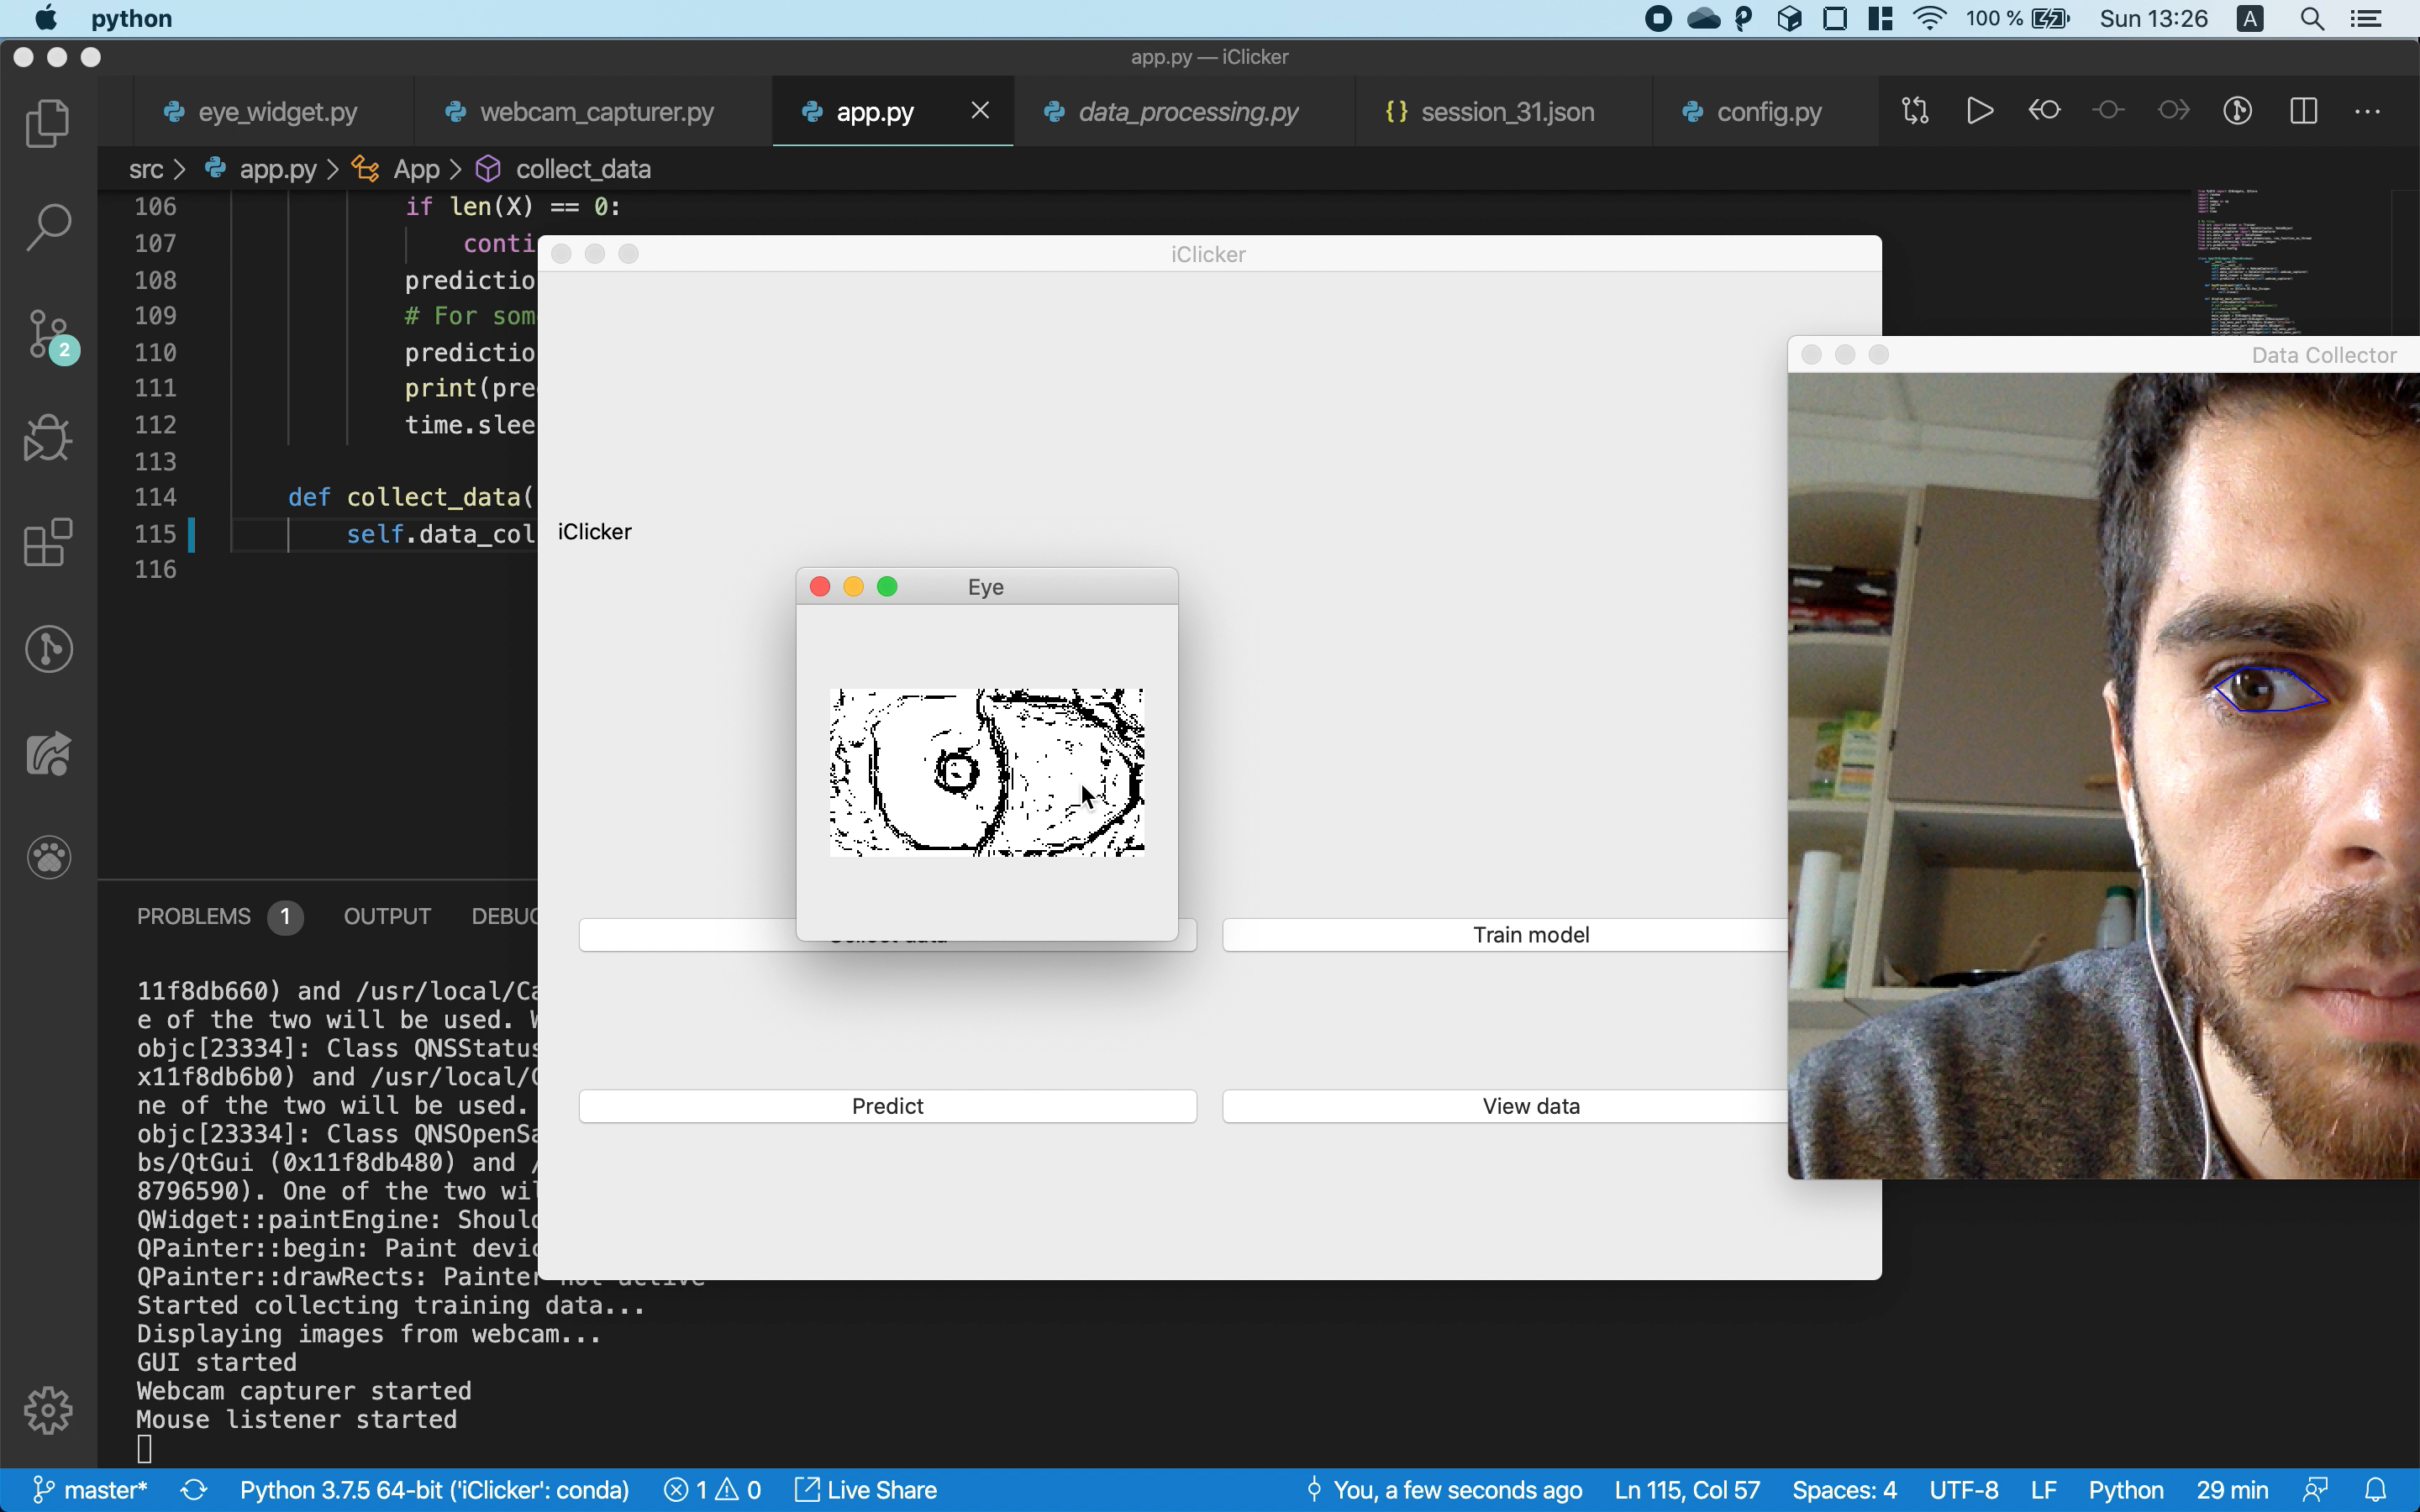
\includegraphics[width=0.5\textwidth]{eye_binary_threshold.png}
    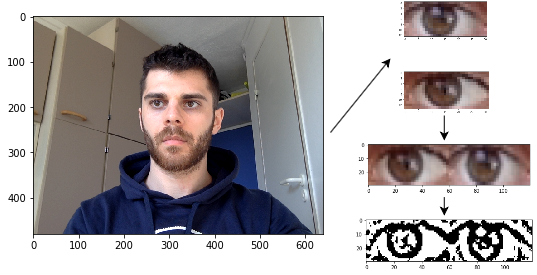
\includegraphics[width=0.5\textwidth]{threshold_process.png}
    \caption{Obținerea de informații din imaginile ochilor}
\end{figure}

\section{Folosirea întregii feți}
\paragraph{}
Următoarea idee a fost să folosesc fața completă a utilizatorului, apoi să o transmit unei rețele neuronale convoluționale.
Procesul de extragere a feței arată astfel:
\begin{figure}[h]
    \centering
    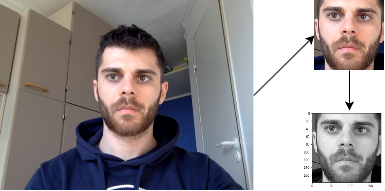
\includegraphics{extract_face_process.png}
    \caption{Extraire le visage}
    \label{fig_extracted_faces}
\end{figure}

\paragraph{}
Imaginea finală este în forma unui pătrat, conținând fața extrasă din imagine, convertită apoi in gri.
Este, de asemenea, normalizată, pentru a lua valori între $0$ și $1$.

\begin{lstlisting}[language=Python, caption=Extragerea feței dintr-o imagine]
def extract_face(cv2_image):
    """Returns the face part extracted from the image"""
    global _face_detector
    if _detectors_are_initialised() == False:
        _initialize_detectors()

    gray_image = Utils.convert_to_gray_image(cv2_image)
    rects = _face_detector(gray_image, 0)
    if len(rects) > 0:
        # only for the first face found
        (x, y, w, h) = face_utils.rect_to_bb(rects[0])
        return cv2_image[y:y+h, x:x+w]
    return None
\end{lstlisting}

\section{``Bandă oculară''}
\paragraph{}
Următoarea opțiune și cea care a rămas integrată în soluția finală a fost să folosesc ambii ochi, fără modificări adiționale.
Procesul de extragere a ochilor arată astfel:

\begin{figure}[h]
    \centering
    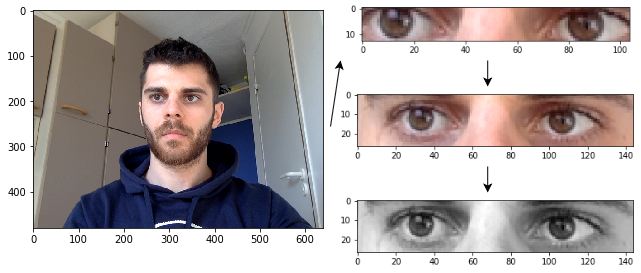
\includegraphics[width = \textwidth]{extract_eye_strip_process.png}
    \caption{Extragerea ``bandei oculare''}
    \label{fig_extracting_eye_strip}
\end{figure}

\paragraph{}
După ce am detectat fața, am extras ambii ochi, am mărit zona dreptunghiulară care încadrează ochii, pentru a avea mai multă informație, apoi am convertit imaginea în gri și am normalizat valorile pixelilor.

\begin{lstlisting}[language=Python, caption=Extragerea ``bandei oculare'' în Python3]
def extract_eye_strip(cv2_image):
    """Returns a horizontal image containing the two eyes extracted from the image"""
    global _face_detector, _face_predictor
    if _detectors_are_initialised() == False:
        _initialize_detectors()

    gray_image = Utils.convert_to_gray_image(cv2_image)
    rects = _face_detector(gray_image, 0)
    if len(rects) > 0:
        # only for the first face found
        shape = _face_predictor(gray_image, rects[0])
        shape = face_utils.shape_to_np(shape)
        (left_eye_start,
         left_eye_end) = face_utils.FACIAL_LANDMARKS_IDXS["left_eye"]
        (right_eye_start,
            right_eye_end) = face_utils.FACIAL_LANDMARKS_IDXS["right_eye"]
        # get the contour
        start, end = min(left_eye_start, right_eye_start), max(
            left_eye_end, right_eye_end)
        strip = shape[start:end]
        # get the upper left point, lower right point
        start = [min(strip, key=lambda x: x[0])[0],
                 min(strip, key=lambda x: x[1])[1]]
        end = [max(strip, key=lambda x: x[0])[0],
               max(strip, key=lambda x: x[1])[1]]
        # go a little outside the bounding box, to capture more details
        distance = (end[0] - start[0], end[1] - start[1])
        # 20 percent more details on the X axis, 60% more details on the Y axis
        percents = [20, 60]
        for i in range(0, 2):
            start[i] -= int(percents[i]/100 * distance[i])
            end[i] += int(percents[i]/100 * distance[i])
        return cv2_image[start[1]:end[1], start[0]:end[0]]
    return None

\end{lstlisting}